% This is based on the LLNCS.DEM the demonstration file of
% the LaTeX macro package from Springer-Verlag
% for Lecture Notes in Computer Science,
% version 2.4 for LaTeX2e as of 16. April 2010
%
% See http://www.springer.com/computer/lncs/lncs+authors?SGWID=0-40209-0-0-0
% for the full guidelines.
%
\documentclass{llncs}
\usepackage[T1]{fontenc}	
\usepackage[utf8]{inputenc}		
\usepackage{graphicx}	
\begin{document}

\title{CBFB: A New Mode of Operation for Byte-Oriented Stream Ciphers}
%
\titlerunning{CBFB}  % abbreviated title (for running head)
%                                     also used for the TOC unless
%                                     \toctitle is used
%
\author{Luiz Augusto Fontes Laranjeira\inst{1} \and Gabriela Matias Navarro\inst{2} }
%
\authorrunning{Ivar Ekeland et al.} % abbreviated author list (for running head)
%
%%%% list of authors for the TOC (use if author list has to be modified)
\tocauthor{Luiz Augusto Fontes Laranjeira and Gabriela Matias Navarro }
%
\institute{University of Brasilia, Brasilia DF 70910-900, BR,\\
\email{luiz.laranjeira@gmail.com}
\and
University of Brasilia, Brasilia DF 70910-900, BR, \\
\email{navarro1703@gmail.com}}%

\maketitle              % typeset the title of the contribution

\begin{abstract}
This paper introduces a new mode of operation for byte-oriented stream ciphers. This mode of operation, which we call CCFB (Ciphertext Byte Frequency Balancing mode), consists of an algorithm that balances out the byte frequency of the ciphertext produced by the stream cipher. The main benefit of its utilization is to make cryptanalysis by means of statistical byte frequency examination of the cipher text more difficult for potential attackers, producing therefore, more secure communications.  
\keywords{stream cipher, cryptography, byte frequency, balance}
\end{abstract}
%
\section{Introduction}
%
The main purpose of the use of cryptography is to keep information confidential, that is, to protect information from non-authorized access by transforming the plaintext into ciphertext and then allowing authorized users to recover the plaintext from the ciphertext, all of this by means of cryptosystems composed of ciphering/deciphering algorithms and one or more keys. There is continuous advancement in the world of cryptography and new algorithms are constantly emerging. Evolution in this field of knowledge is followed closely by the progress of cryptanalysis, which refers to the study of cryptosystems with a view of finding weaknesses in them that might facilitate the retrieval of the plaintext from the ciphertext, without necessarily knowing the key(s) or the algorithm.
%
One of the most well-known methods used in cryptanalysis is the statistical analysis of the byte frequency of a ciphered message. Although this approach was primarily used with classical ciphers, such as the Caesar and Vigenère ciphers, to exploit the character frequency that is inherent to a given written language, it can still be extended and applied to modern block ciphers such as DES and AES[ ], as well as to modern stream ciphers such as SNOW and RC4 [ ].

%
\section{Background}
%
There are two main types of cryptosystems: symmetric key cryptosystems and asymmetric key cryptosystems. An asymmetric key cryptosystem uses a pair of keys, correlated to one another in some mathematical way, such that one of the keys is used to encrypt the plaintext, while the other is used to decrypt the produced ciphertext. A symmetric key cryptosystem uses the same key to encrypt the plaintext and to decrypt the corresponding ciphertext. Symmetric key cryptosystems may use block ciphering/deciphering algorithms or stream ciphering/deciphering algorithms. 
%
Block ciphers encrypt/decrypt an entire block of characters/bytes in a single operation, where the size of each block is predefined. The plaintext is processed block by block in the encryption procedure, as well as in the decryption procedure. Well-known block ciphers are the Data Encryption Standard (DES), developed by IBM, and the Advanced Encryption Standard (AES), developed by two Belgian cryptographers, Joan Daemen and Vincent Rijmen.
%
Stream ciphers can be bit-oriented, byte-oriented or word-oriented, depending on whether they encrypt/decrypt the plaintext/ciphertext one bit, one byte or one word at a time.
\subsection{Stream Ciphers}
%
The stream cipher is the cipher that we used to develop this algorithm. The stream cipher encrypts the text using bit per bit or byte per byte.  It is widely used for network system such as bluetooth and SSL, the reason it is so used is because is faster than the block cipher.

The other advantage is the possibility to transform a block cipher in stream cipher and for that it is needed to set the block size for bit or byte. Nowadays, there are four algorithms that covers 80\% of the world telecommunication and cyber space, they are: A5/1, A5/2, E0 and RC4.(citation BAKHTIARI)

The overall behavior of a stream cipher follows the figure bellow (COLOCAR FIGURA). It encompasses the generation of a random byte keystream (which is generated from a key) and an encryption/decryption function. At the sender side the encryption function, usually an exclusive-or operation, takes as inputs the sequence of bytes of a plaintext and the generated keystream and produces the corresponding ciphered byte sequence. At the receiver side the same keystream must be again generated and the exclusive-or operation once more applied to the ciphertext sequence to recover the plaintext.

This paper presents an application of the byte frequency balancing algorithm that we propose to the RC4 stream cipher. We choose this algorithm because is considered to be the fastest cipher algorithm available. We will explain how this the RC4 works.
%
\subsubsection{RC4}
It was projected by Ron Rivest in 1987 and is widely used, because of its simplicity and high performance, in network systems such as SSL, TLS, WEP, and WPA, as well as in applications like Microsoft Windows, Lotus Notes, Apple AOCE, Oracle and Secure SQL, among others. RC4 employs a variable key size and its operation is based on random permutations of a set of byte values.

It needs a pseudorandom number generator and the permutations are made on those numbers. It reads the plain text byte per byte and encrypts it with the exclusive-or operation. Bellow we can see a pseudo code for this algorithm.

\subsection{Pseudorandom number generator}
The generation of random numbers has been the object of attention of mathematician for many years. The main problem for a long time was to produce a deterministic algorithm with a sufficiently long periodicity as to simulate an apparently-random sequence of values to be used by complex applications.

Although the so-called True Random Number Generators (TRNGs)  exist and produce a sequence of numbers that are really random, in the case of applications such as cryptography one needs to be able to produce the same sequence of random numbers when performing both encryption as well as decryption. As a consequence, this sequence of numbers must be generated in a deterministic manner by the so-called PseudoRandom Number Generators (PRNGs).

Many PRNG algorithms have been designed and are widely used in cryptography, in particular in the implementation of stream ciphers. To be considered a pseudorandom number generator, the produced sequence must follow two criteria: 

Randomness: the main requirement to make sure the sequence is random is to be sure that the numbers are random. It also have two criteria to validate this:
	Uniform distribution: the frequency of bits in the sequence must approximately be the same, therefore, the amount of 0 must be approximate to the amount of 1.
	Independence: the numbers don't have relation between them.

Unpredictability: This assure that if you know any number from the sequence, you can't predict the previous or the later number. 

We will use the RC4 for byte random generation.

\subsubsection{RC4}

Although the RC4 is most know as a cipher algorithm, it is also a strong pseudo random generator. It is based on permutation of the 255 available bytes. There are two steps that needs to be done to make this algorithm work. 

\subsubsection{Key Inicialization}
This algorithm accepts any size of key. The first thing is done is inicialization of the vector S. This vector has size of 255 and to initialize each position of this vector is set equal to the corresponding character. For example: S[0] = 0, S[1] = 1 .... S[255] = 255. At the same time, another vector is created. This is a temporary vector, so we will call it T. If the key has size 256 bytes, we make T equal to K. But if the key is less than 256 bytes, the key is repeated until it completes the 256 position of the T vector.

This temporary vector is used to make the first permutation of the S vector. For this, we will use two control variables: i and j, and i goes from 0 to 255. At this point we will only swap the value contained in S[i] to S[j]. And the value contained in S[j] to S[i].

The following rule is used to make this permutation is:

\begin{equation}
  j := (j + S[i] + T[i]) mod 256
\end{equation}

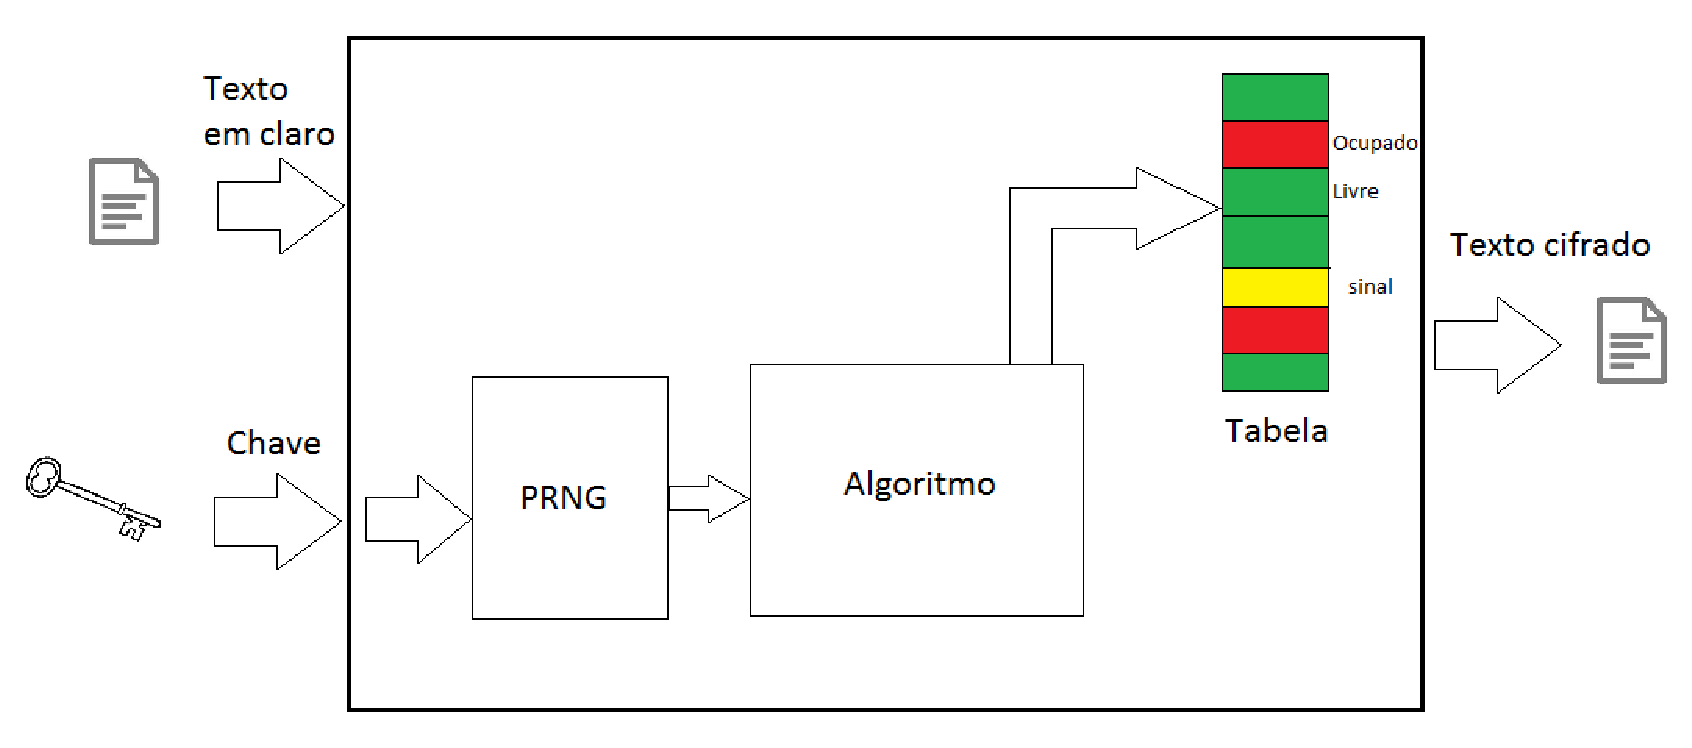
\includegraphics{./figuras/funcionamento}

\subsubsection{Char generation}

After the key inicialization and S is initialized, it's time to generate characters to use in the cipher process. This process still uses the control variable i and j and the both starts with 0. This generation is made by using the following equation:

\begin{equation}
 i := (i + 1) mod 256
\end{equation}

\begin{equation}
 j := (j + S[i]) mod 256
\end{equation}

After this two variables are obtained a swap operation is done with the values of S[i] and S[j]. And the following operation is done:

\begin{equation}
 t := (S[i] + S[j]) mod 256
\end{equation}

The character generated is equal to S[k].

\section{The algorithm}

This section will present the algorithm that we aim to propose, details of its functioning and advantages.

\subsection{Motivation}

The evolution in cryptography is constant and there are always new algorithms that focus in create a solution of a new obstacles that are imposed by possible attackers and their methods to obtain secret informations. 

This algorithm want to create a solution for a well known problem with cryptography. It wants to  reduce  the possibilities to obtain a secret information by using frequency analysis.

\subsection{Functioning}

The cipher algorithm will receive a plain text and a sequence of pseudorandom numbers will produce a cipher text where all the bytes frequency occurrence will be balanced.

The mechanism that will be used to produce this balancing is in form of rounds of 256 bytes that each byte will appear only once in each round.  That means that the 256 cipher bytes of each round are distinct, but the order that it appear is pseudorandom.

A table of 256 bytes will be used to make the balancing of the cipher text. In the beginning of the round of all 256 positions are set to not occupied. For each byte of the plain text will cipher will be transform by a exclusive-or operation with the corresponding value supplied from the pseudorandom number generator resulting in a preciphered byte. With this preciphered byte the algorithm will check if the value is occupied on the table.After the balancing table is completed, the table is reset and the process starts over.

In case this preciphered byte is equal to a position already occupied on the table, this value will be rejected and the next value of the pseudorandom sequence will be use to make a new cipher text for that plain text byte. This procedure will be repeated until a non occupied position at the table is achieved. The amount of unused pseudorandom numbers will be recorded in a variable called j. This variable will be set to 0 again when the preciphered byte is equal to a non occupied value on the table.

A control variable called signal is used so that the decipher can know that a conflict existed at some point. In this way, the decipher can know that the following byte is another control variable and will represent the amount of characters that needs to be discarded ( the j variable ). The signal variable is not ciphered, because in this way, all the 256 bytes can be used to cipher.

On the decipher algorithm the balancing table is not needed and therefore not used. On every round, the first value of the pseudorandom generator character is set to be the signal of the round. Because of this, a control variable needs to be used to know when is need to get a new signal.


\section{Results}

To make a more realistic approach, it was used a network connection (TCP) with the code of the algorithm here proposed. 

The scheme that was used can be seen on the bellow image. A message queue was used so that the cipher routine could put the ciphertext byte on the message queue.

MAKE A IMAGE SHOWING THE ARCHITECTURE

Another feature that was also used is a  thread, that was responsible to send the values from the queue to the decipher algorithm. 

The table bellow shows some results of experiments that was performed with the code produced following the above architecture.

PUT TABLE


\section{Conclusion}



%
% ---- Bibliography ----
%
\begin{thebibliography}{5}
%
\bibitem {clar:eke}
Clarke, F., Ekeland, I.:
Nonlinear oscillations and
boundary-value problems for Hamiltonian systems.
Arch. Rat. Mech. Anal. 78, 315--333 (1982)

\bibitem {clar:eke:2}
Clarke, F., Ekeland, I.:
Solutions p\'{e}riodiques, du
p\'{e}riode donn\'{e}e, des \'{e}quations hamiltoniennes.
Note CRAS Paris 287, 1013--1015 (1978)

\bibitem {mich:tar}
Michalek, R., Tarantello, G.:
Subharmonic solutions with prescribed minimal
period for nonautonomous Hamiltonian systems.
J. Diff. Eq. 72, 28--55 (1988)

\bibitem {tar}
Tarantello, G.:
Subharmonic solutions for Hamiltonian
systems via a $\bbbz_{p}$ pseudoindex theory.
Annali di Matematica Pura (to appear)

\bibitem {rab}
Rabinowitz, P.:
On subharmonic solutions of a Hamiltonian system.
Comm. Pure Appl. Math. 33, 609--633 (1980)

\end{thebibliography}

\end{document}
